\section{Rich Picture}

\begin{figure}[H]
    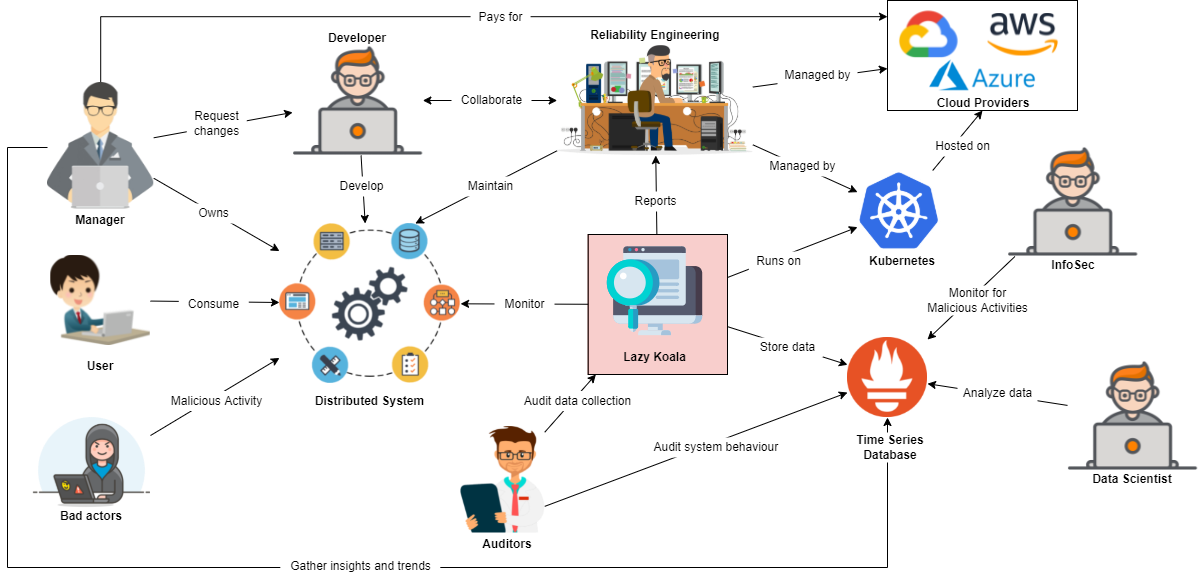
\includegraphics[width=16cm]{assets/requirement-specification/rich-picture.png}
    \caption{Rich picture diagram (self-composed)}
    \label{fig:rich-picture}
\end{figure}

The purpose of this project is to create an AI-powered monitoring system that will help \acp{sres} to detect and diagnose issues in the system quickly. The flow of the system goes as follows, The manager requests the development team to create a software to full fill a customer's need. Then the development team will develop the software and with the help of \acp{sres} the software will be deployed for public use. After that, it's \acp{sres} due to keeping the system up and running while doing routine maintenance. While the software is running another monitoring system will keep an eye on its health and general behavior. If one or more components of the system try to deviate from its regular behavior it's the monitoring system's job to notify \acp{sres} of a few possible reasons for this unexpected behavior. Finally, \acp{sres} and the development team will launch a coordinated effort to identify the real issue and resolve it quickly as possible. 